\begin{frame}{Direct Detection mit Flavour-Mischung}
	Annahmen: DM koppelt ausschließlich an $Z'$. Von den Quarks wechselwirken nur $s,b$ mit $Z'$. \\
	\resizebox{.5\textwidth}{!}{
		\begin{tikzpicture}
\tikzstyle{centerArrow}=[decoration={
markings,
mark=at position 0.5 with {\fill (2pt,0)--(-2pt,2.31pt)--(-2pt,-2.31pt)--cycle;}}]
\begin{scope}[xshift=3cm,yshift=-2cm]
\def\xmove{2}
\def\ymove{1.25}
\def\centerShift{2}
\def\centerSize{0.08cm}
\coordinate (tCenter1) at (0,0);
\coordinate[fill, circle,inner sep=\centerSize] (tCenter2) at (0,-\centerShift cm);
\node (upperLeft) at (-\xmove,\ymove) {$\chi$};
\node (upperRight) at (\xmove,\ymove) {$\chi$};
\node (lowerLeft) at (-\xmove,-\centerShift cm-\ymove cm) {$b_L,s_L$};
\node (lowerRight) at (\xmove,-\centerShift cm-\ymove cm) {$s_L,b_L$};
\node at (0.5,-\centerShift/2) {$Z'$};
\draw [centerArrow,postaction={decorate}]  (upperLeft) -- (tCenter1) ;
\draw [centerArrow,postaction={decorate}]  (tCenter1) -- (upperRight) ;
\draw [centerArrow,postaction={decorate}]  (lowerLeft) -- (tCenter2) ;
\draw [centerArrow,postaction={decorate}]  (tCenter2) -- (lowerRight) ;
\draw [decoration={snake, segment length=1.5mm, amplitude=0.5mm},decorate] (tCenter1) -- (tCenter2) ;
\end{scope}
\end{tikzpicture}
	}
\end{frame}


\begin{frame}{Schranken aus dem $B$-Zerfall 1}
\framesubtitle{Real- und Imaginärteil variabel}
	\begin{figure}
		\centering
		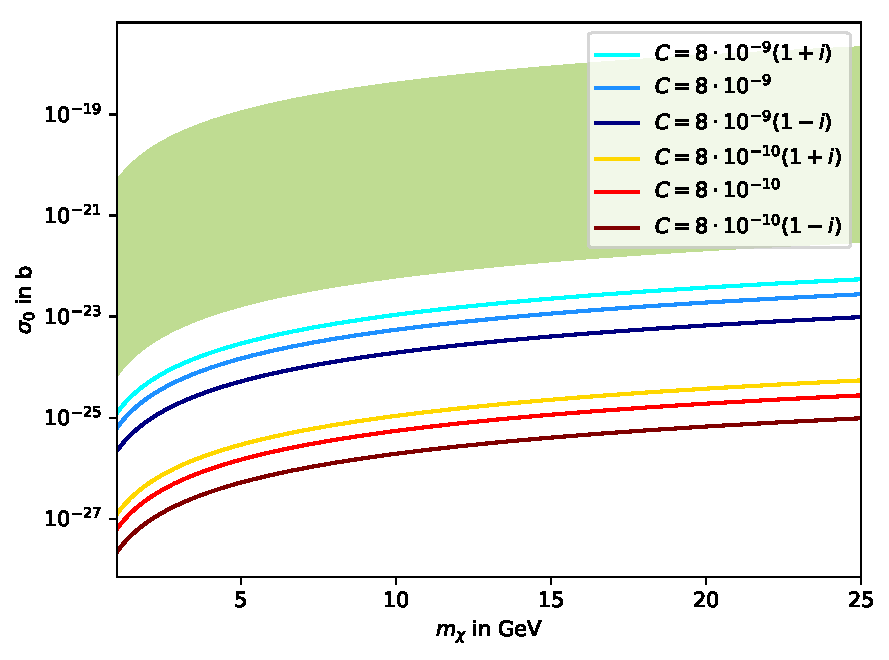
\includegraphics[width=.8\textwidth]{Bilder/Allgemein11.pdf}
		\caption{$q_l=q_\chi=1$}
	\end{figure}
\end{frame}
\begin{frame}[noframenumbering]{Schranken aus dem $B$-Zerfall 1}
\framesubtitle{Real- und Imaginärteil variabel}
	\begin{figure}
		\centering
		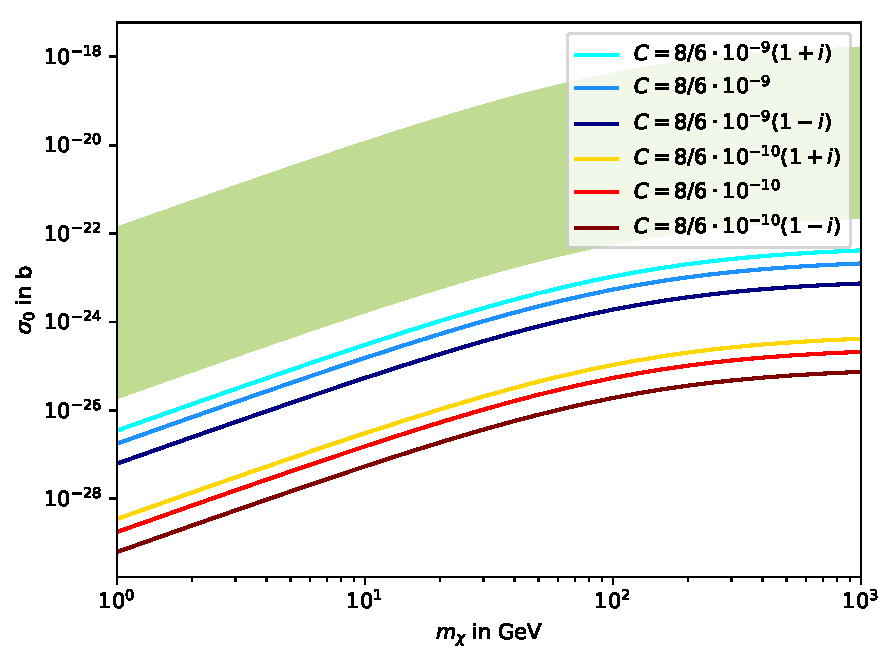
\includegraphics[width=.8\textwidth]{Bilder/Allgemein116.pdf}
		\caption{$q_l=1,q_\chi=\sfrac{1}{6}$}
	\end{figure}
\end{frame}


\begin{frame}{Schranken aus dem $B$-Zerfall 2}
\framesubtitle{Fester Realteil, variabler Imaginärteil}
	\begin{figure}
		\centering
		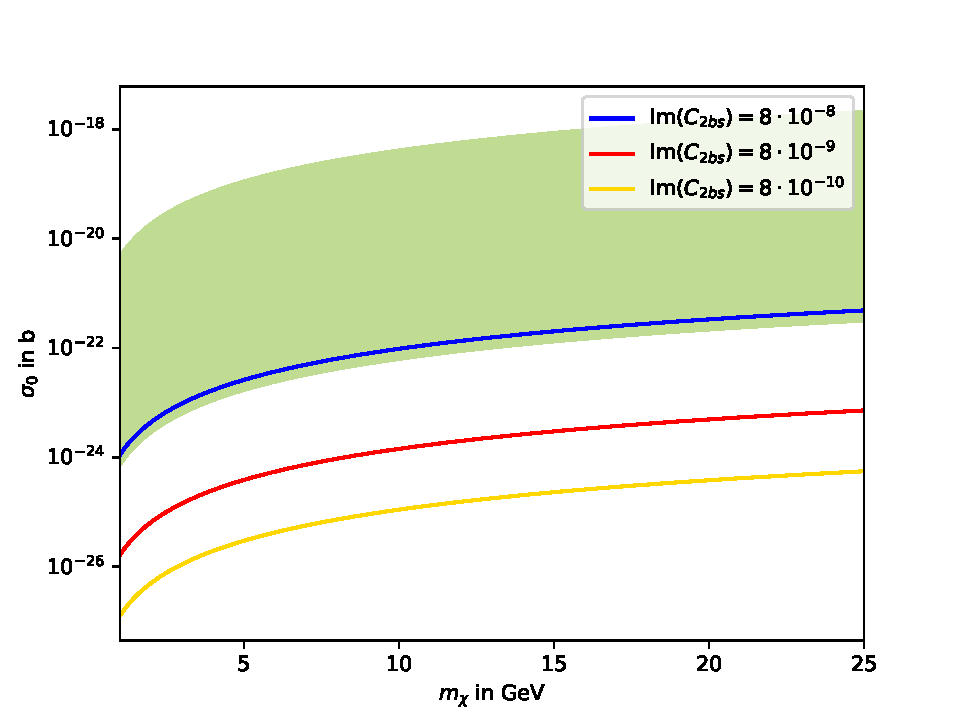
\includegraphics[width=.8\textwidth]{Bilder/Im11.pdf}
		\caption{$q_l=q_\chi=1$}
	\end{figure}
\end{frame}
\begin{frame}[noframenumbering]{Schranken aus dem $B$-Zerfall 2}
\framesubtitle{Fester Realteil, variabler Imaginärteil}
	\begin{figure}
		\centering
		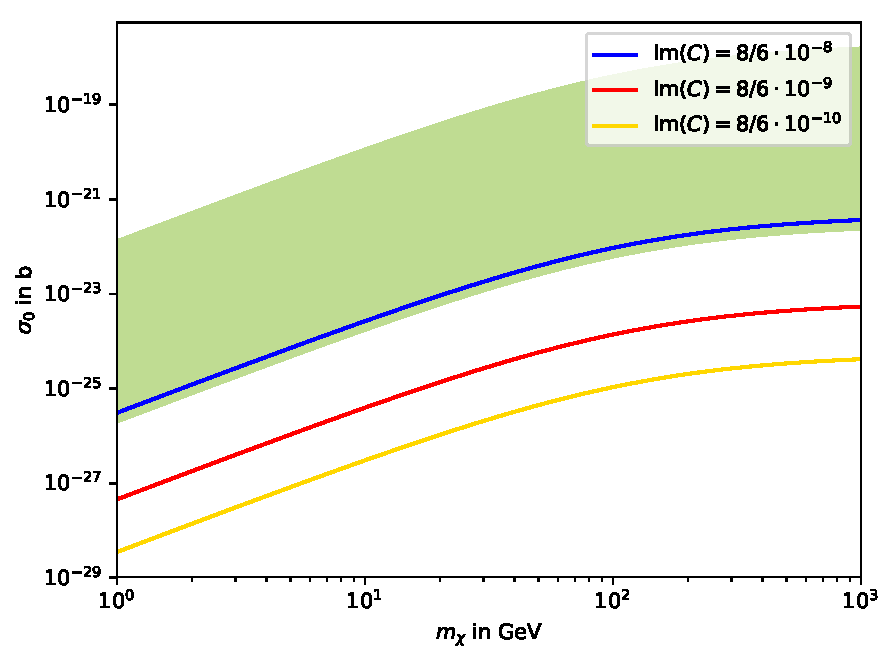
\includegraphics[width=.8\textwidth]{Bilder/Im116.pdf}
		\caption{$q_l=1,q_\chi=\sfrac{1}{6}$}
	\end{figure}
\end{frame}


\begin{frame}{Schranken aus der Relic Density}
\begin{figure}
	\centering
	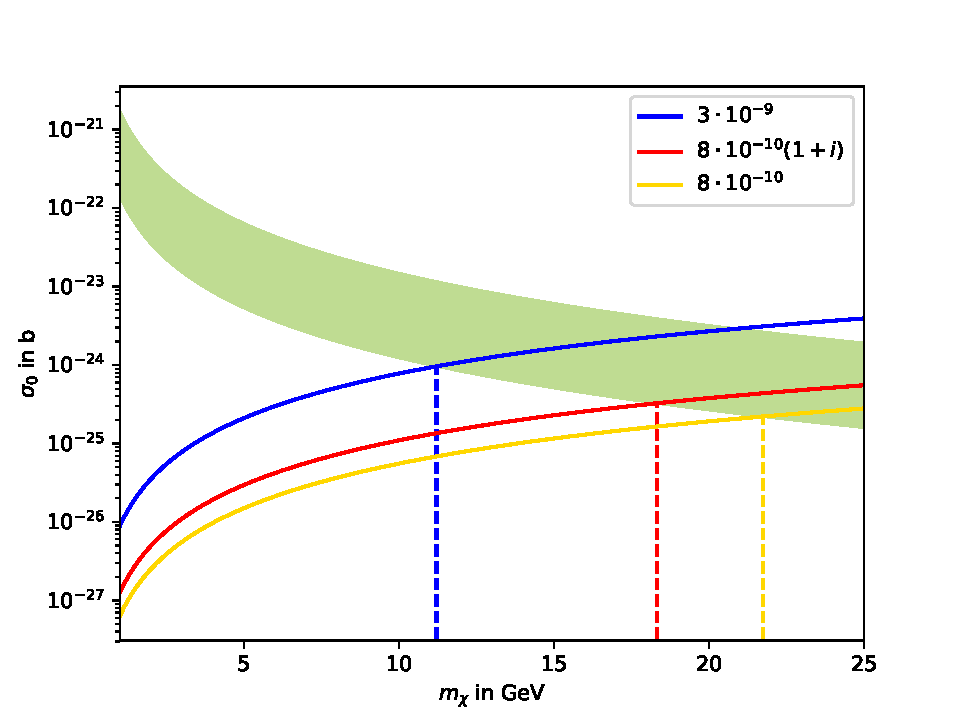
\includegraphics[width=.8\textwidth]{Bilder/Relic11.pdf}
	\caption{$q_l=q_\chi=1$}
\end{figure}
\end{frame}
\begin{frame}[noframenumbering]{Schranken aus der Relic Density}
\begin{figure}
\centering
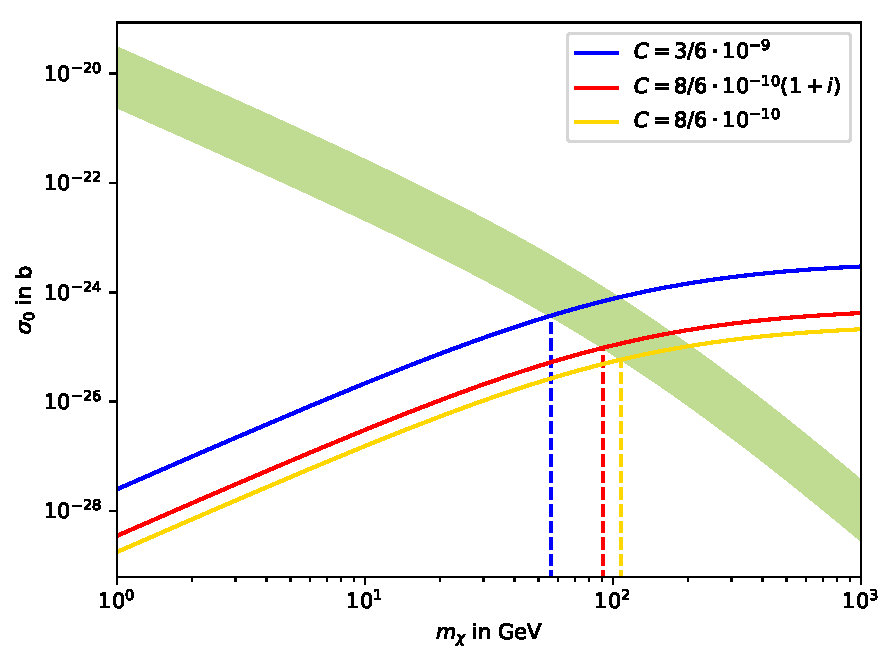
\includegraphics[width=.8\textwidth]{Bilder/Relic116.pdf}
\caption{$q_l=1,q_\chi=\sfrac{1}{6}$}
\end{figure}
\end{frame}